% Compile with pdfLaTeX. All figures are included in this source.
% This researcher-facing report contains case answers.
\documentclass[10pt,a4paper]{article}
\usepackage[T1]{fontenc}
\usepackage[utf8]{inputenc}
\usepackage{lmodern,microtype}
\usepackage[margin=20mm,headheight=14pt]{geometry}
\usepackage[table]{xcolor}
\usepackage{booktabs,tabularx,array,amsmath,tikz,fancyhdr,hyperref}
\usetikzlibrary{arrows.meta,positioning,calc}
\definecolor{Ink}{HTML}{19334B}
\definecolor{Teal}{HTML}{087F8C}
\definecolor{Blue}{HTML}{3568A3}
\definecolor{Purple}{HTML}{8064A2}
\definecolor{Amber}{HTML}{BF7A27}
\definecolor{Muted}{HTML}{52616B}
\hypersetup{colorlinks=true,linkcolor=Teal,urlcolor=Teal,pdftitle={UC-Bench: evaluating AI agents that assess treatment-response predictors}}
\pagestyle{fancy}\fancyhf{}
\fancyhead[L]{\small UC-Bench: treatment-response studies}
\fancyhead[R]{\small September 2026}
\fancyfoot[L]{\scriptsize Controlled research exercises, not clinical validation}
\fancyfoot[R]{\thepage}
\setlength{\parindent}{0pt}
\setlength{\parskip}{5pt}
\setlength{\emergencystretch}{2em}
\renewcommand{\arraystretch}{1.2}
\newcolumntype{Y}{>{\raggedright\arraybackslash}X}
\newcommand{\reportcase}[2]{{\Large\bfseries Case #1. #2\par}\vspace{2mm}}
\newcommand{\reporthead}[1]{\vspace{2mm}{\normalsize\bfseries #1\par}}
\newcommand{\reportcaption}[1]{\par{\small\color{Muted}#1\par}\vspace{1mm}}
\newcommand{\reportstatus}[1]{{\small\color{Muted}#1\par}\vspace{1mm}}
\newcommand{\reportmet}{\cellcolor{Teal!18}Met}
\newcommand{\reportfailed}{\cellcolor{Amber!23}Failed}
\newcommand{\reportmissing}{\cellcolor{black!8}Missing}
\newcommand{\reportunscored}{\cellcolor{black!8}--}
\tikzset{
 box/.style={draw=Ink!60,fill=Teal!5,rounded corners=2pt,align=center,font=\small,text width=12cm,minimum height=8mm,inner sep=4pt},
 gate/.style={box,fill=Amber!10,draw=Amber},
 result/.style={box,fill=Teal!10,draw=Teal},
 arr/.style={-{Latex[length=1.8mm]},thick,draw=Ink!80},
 dep/.style={arr,dashed,draw=Muted}
}
\begin{document}
{\LARGE\bfseries Evaluating AI agents that assess treatment-response predictors\par}
\vspace{2mm}
A research team receives a predictor that estimates which patients will improve after infliximab treatment for ulcerative colitis. The team must decide whether to fund another study, request missing information or stop the proposed use. A high reported accuracy is not enough. The team must check the patient records, reproduce the calculations and determine what the results actually support.

UC-Bench gives that investigation to an AI agent. The report calls these agents Models 1--4. They are separate from the treatment-response predictor that they inspect. The predictor stays fixed. The agent's task is to assess it, not replace it.

\reporthead{What happens in one attempt}
The agent receives patient records, predicted response chances, study documents and processing records. It can read files, write code and save calculations. The environment initially hides the patients' response results. The agent must record its patient selection and analysis plan before it receives those results.

\begin{center}
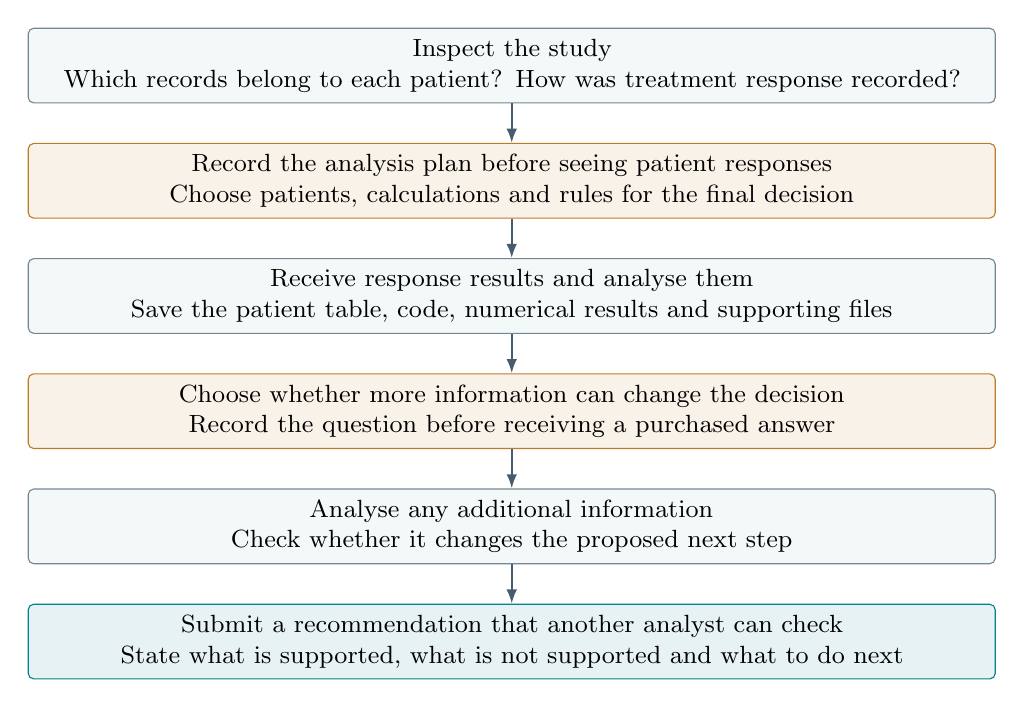
\begin{tikzpicture}[node distance=5mm]
\node[box] (a) {Inspect the study\\Which records belong to each patient? How was treatment response recorded?};
\node[gate,below=of a] (b) {Record the analysis plan before seeing patient responses\\Choose patients, calculations and rules for the final decision};
\node[box,below=of b] (c) {Receive response results and analyse them\\Save the patient table, code, numerical results and supporting files};
\node[gate,below=of c] (d) {Choose whether more information can change the decision\\Record the question before receiving a purchased answer};
\node[box,below=of d] (e) {Analyse any additional information\\Check whether it changes the proposed next step};
\node[result,below=of e] (f) {Submit a recommendation that another analyst can check\\State what is supported, what is not supported and what to do next};
\foreach \x/\y in {a/b,b/c,c/d,d/e,e/f} \draw[arr] (\x)--(\y);
\end{tikzpicture}
\end{center}
\reportcaption{Figure 1. The investigation shared by all four cases.}

The agent can buy at most one information package within a small simulated budget. Options include checking patient identities, reviewing response records, executing analysis code, obtaining another study's data, increasing sample size or requesting expert review. It can also buy nothing. The correct choice depends on which answer would change the next research decision.

\reporthead{How the cases connect}
Case 1 asks whether a study can proceed despite a limited documentation problem. Case 2 asks whether the result persists when repeated patients and study sites are examined. Case 3 asks whether the predictions came from a procedure that can be checked. Case 4 asks whether useful patient ranking also supports decisions based on predicted chances.

These are separate investigations within one environment, not successive studies of the same patients. Cases 1 and 2 contain observed agent results. Cases 3 and 4 describe further studies and their available reference calculations.

\reporthead{How to read the results}
A \textbf{complete investigation passes} only when the agent submits and meets every essential check. The \textbf{work score}, from 0 to 100, credits calculations and decisions that the evaluator can verify. Finishing and being correct are separate outcomes. The evaluator recalculates important numbers from saved files rather than accepting the agent's reported answer.

\newpage
\reportcase{1}{Can the study proceed with its current records?}
\reportstatus{Observed results from four AI agents. One attempt per agent.}
The first case asks the agent to make a limited research decision. Does the study justify another stage of testing, or must the team obtain more information first? It does not ask whether the predictor is ready for patient care.

The packet contains 134 records from 124 people. Some people therefore contribute more than one record. The agent must identify those records so that it does not count one person several times. One included patient's response also has uncertain documentation. The question is whether the recorded response has a sufficiently supported source.

\reporthead{The work behind the decision}
The agent first chooses which patients to include and how to handle repeated records. It records those choices before it receives the response results. It then checks whether the predicted chances distinguish responders from nonresponders and whether results vary across study sites. It also checks how uncertain the estimates are and what errors the proposed decision rule would make.

\begin{center}
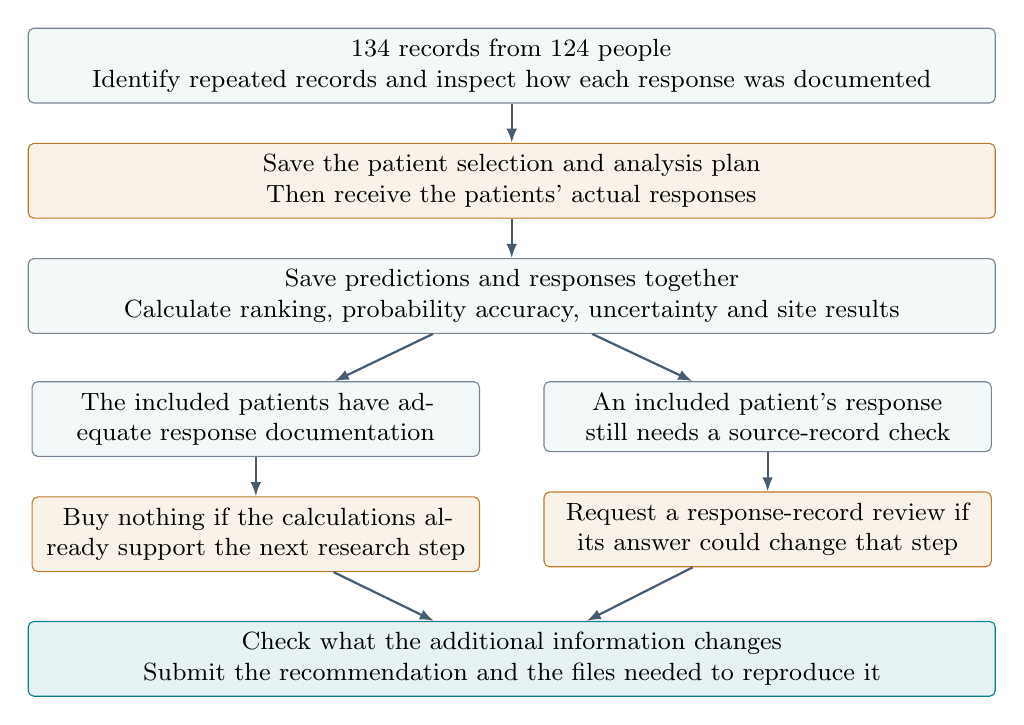
\begin{tikzpicture}[node distance=5mm]
\node[box] (a) {134 records from 124 people\\Identify repeated records and inspect how each response was documented};
\node[gate,below=of a] (b) {Save the patient selection and analysis plan\\Then receive the patients' actual responses};
\node[box,below=of b] (c) {Save predictions and responses together\\Calculate ranking, probability accuracy, uncertainty and site results};
\node[box,text width=5.4cm,below=6mm of c.south,xshift=-3.25cm] (d) {The included patients have adequate response documentation};
\node[box,text width=5.4cm,below=6mm of c.south,xshift=3.25cm] (e) {An included patient's response still needs a source-record check};
\node[gate,text width=5.4cm,below=of d] (f) {Buy nothing if the calculations already support the next research step};
\node[gate,text width=5.4cm,below=of e] (g) {Request a response-record review if its answer could change that step};
\node[result,anchor=north] (h) at ($(f.south)!0.5!(g.south)+(0,-.65)$) {Check what the additional information changes\\Submit the recommendation and the files needed to reproduce it};
\foreach \x/\y in {a/b,b/c,c/d,c/e,d/f,e/g,f/h,g/h} \draw[arr] (\x)--(\y);
\end{tikzpicture}
\end{center}
\reportcaption{Figure 2. Case 1's patient and documentation decisions.}

A response-record review checks the source behind the recorded responder/nonresponder result. It can resolve a documentation problem without changing that result. This matters because an unchanged number can become better supported.

Both successful agents justified a 123-person analysis before seeing responses. They did not need an additional purchase for their immediate decision. An agent that retains all 124 people can instead justify the response-record review. The task does not require one patient selection or one purchase.

The final recommendation must remain limited. Support for another research study does not establish support for treatment selection, routine clinical use or use in a different population.

\newpage
\reportcase{1}{Two agents completed the investigation correctly}
\begin{center}
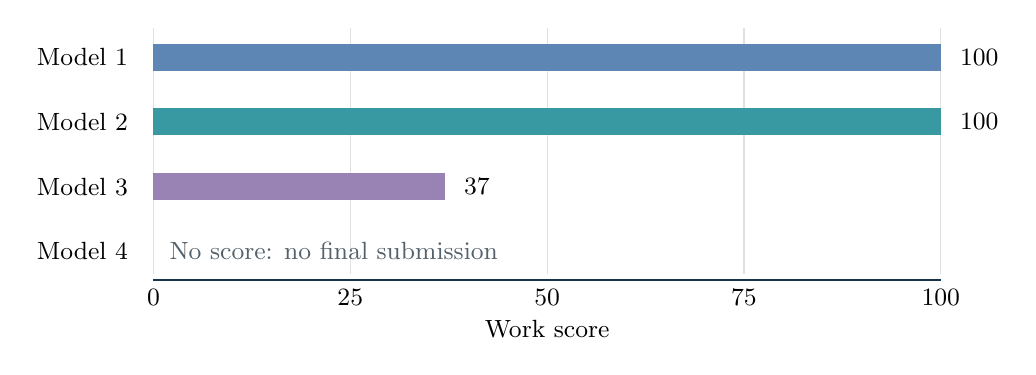
\begin{tikzpicture}[x=1cm,y=.82cm]
\foreach \x in {0,2.5,5,7.5,10} {\draw[black!12] (\x,-.35)--(\x,3.45);}
\foreach \y/\name/\value/\col in {3/Model 1/100/Blue,2/Model 2/100/Teal,1/Model 3/37/Purple} {
 \node[anchor=east,font=\small] at (-.2,\y) {\name};
 \fill[\col!80] (0,{\y-.21}) rectangle ({\value/10},{\y+.21});
 \node[anchor=west,font=\small] at ({\value/10+.12},\y) {\value};
}
\node[anchor=east,font=\small] at (-.2,0) {Model 4};
\node[anchor=west,font=\small,color=Muted] at (.08,0) {No score: no final submission};
\draw[Ink] (0,-.45)--(10,-.45);
\foreach \x/\label in {0/0,2.5/25,5/50,7.5/75,10/100} \node[below,font=\small] at (\x,-.45) {\label};
\node[below,font=\small] at (5,-.92) {Work score};
\end{tikzpicture}
\end{center}
\reportcaption{Figure 3. Verified work in Case 1.}

Models 1 and 2 passed the complete investigation. Model 3 submitted a recommendation but failed essential checks. Model 4 did not submit. The Case 1 scoring method does not assign a work score to that unfinished attempt. A missing bar does not mean zero scientific ability.

\begin{tabularx}{\textwidth}{@{}Ylrr@{}}\toprule
Agent & Final outcome & API requests & Cost (USD) \\\midrule
Model 1 & Complete investigation passed & 47 & 0.58 \\
Model 2 & Complete investigation passed & 48 & 0.79 \\
Model 3 & Submitted, but failed checks & 62 & 8.94 \\
Model 4 & Did not submit & 65 & 1.05 \\\bottomrule
\end{tabularx}
\reportcaption{Table 1. Completion and inference cost.}

\reporthead{What the successful agents found}
Both successful agents analysed 123 people. Both found that responders usually received higher predicted chances than nonresponders. This ranking ability is measured by \textbf{AUC}. An AUC of 0.50 corresponds to chance ranking, while 1.00 indicates perfect ranking. Both agents calculated 0.785.

A study of this size does not determine the ranking score exactly. Model 1 reported a 90\% uncertainty interval of 0.720--0.849. Model 2 used a 95\% interval and obtained 0.697--0.855. These intervals differ because the agents committed to different valid settings.

\begin{tabularx}{\textwidth}{@{}Yrr@{}}\toprule
Question answered by the calculation & Model 1 & Model 2 \\\midrule
How well did the predictor rank patients? AUC & 0.785 & 0.785 \\
How wrong were its probabilities? Brier score & 0.191 & 0.191 \\
How closely did chances match response rates? Calibration error & 0.062 & 0.096 \\
How did the 50\% cutoff perform? Net benefit & 0.171 & 0.171 \\
How well did it rank patients at the weakest site? AUC & 0.694 & 0.694 \\\bottomrule
\end{tabularx}
\reportcaption{Table 2. Results from the two successful investigations.}

The \textbf{Brier score} measures squared probability error, with smaller values indicating less error. \textbf{Calibration} asks whether predicted chances match observed response rates. For example, about 80\% of patients assigned an 80\% chance should respond. The agents used different accepted calibration settings.

\textbf{Net benefit} evaluates a rule that flags patients above a chosen probability cutoff. It rewards correct positive predictions and penalizes incorrect ones under a stated cost rule. Positive values here are relative to flagging nobody. They do not establish clinical benefit.

Both agents recommended further research and bought no additional information. Neither recommended unrestricted clinical use.

\newpage
\reportcase{1}{Why the other investigations did not pass}
The next map shows what the evaluator checked, not ten unrelated administrative requirements. Each row describes a step needed to support the recommendation. A failed result can follow from an earlier missing link.

\begin{tabularx}{\textwidth}{@{}Yccc@{}}\toprule
What the evaluator checked & Model 1 & Model 2 & Model 3 \\\midrule
Kept the plan fixed after seeing responses & \reportmet & \reportmet & \reportmet \\
Linked results to the correct saved calculations & \reportmet & \reportmet & \reportfailed \\
Handled repeated records from the same patient & \reportmet & \reportmet & \reportmet \\
Supported patient ranking and its uncertainty & \reportmet & \reportmet & \reportfailed \\
Supported the checks of predicted chances & \reportmet & \reportmet & \reportfailed \\
Supported the check of the 50\% cutoff & \reportmet & \reportmet & \reportfailed \\
Supported the results for each study site & \reportmet & \reportmet & \reportfailed \\
Interpreted the purchased information correctly & \reportmet & \reportmet & \reportfailed \\
Kept stated confidence consistent with the findings & \reportmet & \reportmet & \reportmet \\
Supported the proposed next research step & \reportmet & \reportmet & \reportfailed \\\bottomrule
\end{tabularx}
\reportcaption{Figure 4. Checks on the completed Case 1 investigations.}

Green means the check passed. Amber means it failed. Model 4 has no completed scientific assessment and does not appear in this map. A failed numerical check does not necessarily mean incorrect arithmetic. The evaluator must also be able to find and reproduce the calculation.

\reporthead{Model 3: a recommendation that could not be reproduced}
Model 3 saved a valid patient table. However, it linked required numerical results to the wrong saved files. This was the first important error. The evaluator could not reproduce the calculations referenced by the recommendation.

\begin{center}
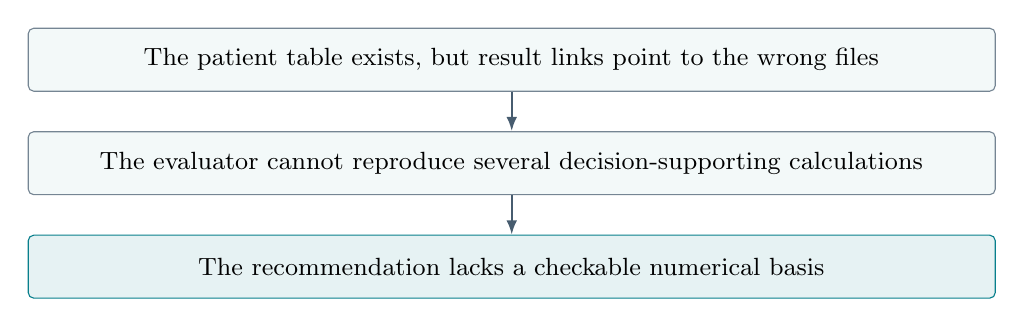
\begin{tikzpicture}[node distance=5mm]
\node[box] (a) {The patient table exists, but result links point to the wrong files};
\node[box,below=of a] (b) {The evaluator cannot reproduce several decision-supporting calculations};
\node[result,below=of b] (c) {The recommendation lacks a checkable numerical basis};
\draw[arr] (a)--(b);\draw[arr] (b)--(c);
\end{tikzpicture}
\end{center}
\reportcaption{Figure 5. One error caused several downstream failures.}

The agent also used incorrect parameter fields for some calculations. Separately, it purchased a response-record review and then said the review changed nothing important. The response labels stayed unchanged, but the review resolved the uncertainty about their source. That was a mistake about the information's meaning, not its arithmetic.

\reporthead{Model 4: the investigation did not reach a recommendation}
Model 4 continued correcting its calculations until it reached the response limit. It did not submit the required final recommendation. The record identifies a completion failure. It does not identify a specific misunderstanding of the biology.

\reporthead{What this establishes}
Case 1 shows that two agents can complete the task without unnecessary purchases. It also shows a failure to maintain reproducible results and a separate failure to interpret a record review. A file-link checker or targeted expert review could help, but neither remedy was tested.

These are four individual attempts, not estimates of long-run success rates. Case 2 next examines whether an apparently useful result survives a more difficult patient and site analysis.

\newpage
\reportcase{2}{Does the result hold within each study site?}
Case 1 allowed a supported next research step. Case 2 presents a different problem: the headline result may hide weak performance within the places that recruited patients. The agent must look beyond the result from the combined sample.

The packet contains 203 records assigned to 96 provisional patient groups. Each group is intended to represent one person. Some groups contain multiple records. The study sites also contribute different numbers of records and patients. Counting every record as an independent person would exaggerate the amount of information.

\reporthead{What the agent must find out}
The agent identifies which records belong to the same patient, chooses the included patients and records its plan before seeing responses. It then compares performance across all patients with performance within each site. A predictor can appear useful in the combined sample even if it ranks patients poorly within individual sites.

\begin{center}
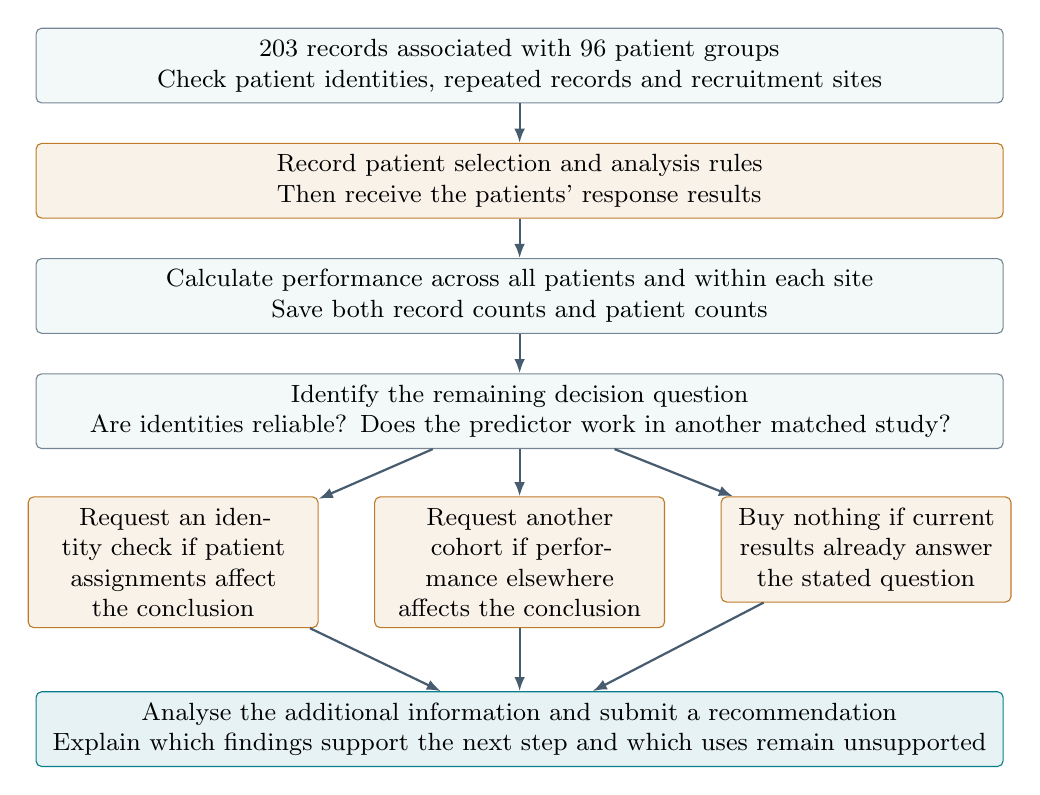
\begin{tikzpicture}[node distance=5mm]
\node[box] (a) {203 records associated with 96 patient groups\\Check patient identities, repeated records and recruitment sites};
\node[gate,below=of a] (b) {Record patient selection and analysis rules\\Then receive the patients' response results};
\node[box,below=of b] (c) {Calculate performance across all patients and within each site\\Save both record counts and patient counts};
\node[box,below=of c] (d) {Identify the remaining decision question\\Are identities reliable? Does the predictor work in another matched study?};
\node[gate,text width=3.4cm,below=6mm of d.south,xshift=-4.4cm] (e) {Request an identity check if patient assignments affect the conclusion};
\node[gate,text width=3.4cm,below=6mm of d.south] (f) {Request another cohort if performance elsewhere affects the conclusion};
\node[gate,text width=3.4cm,below=6mm of d.south,xshift=4.4cm] (g) {Buy nothing if current results already answer the stated question};
\node[result,below=8mm of f] (h) {Analyse the additional information and submit a recommendation\\Explain which findings support the next step and which uses remain unsupported};
\foreach \x/\y in {a/b,b/c,c/d,d/e,d/f,d/g,e/h,f/h,g/h} \draw[arr] (\x)--(\y);
\end{tikzpicture}
\end{center}
\reportcaption{Figure 6. Case 2's patient, site and purchase decisions.}

Agents can use different supported ways to handle repeated records. One approach combines a patient's records. Another retains them but accounts for their shared patient identity. The important requirement is not one fixed method. It is avoiding false confidence from treating dependent observations as independent.

A cohort is a group of patients studied together. An identity check and another cohort answer different questions. Checking identities does not demonstrate performance in a new study. Obtaining another study does not repair an invalid patient selection. The agent must state what a purchase can change before it sees the result.

A recommendation to stop or pause can be correct. However, the agent still needs the calculations and patient records that justify it.

\newpage
\reportcase{2}{Substantial partial work, but no complete success}
\begin{center}
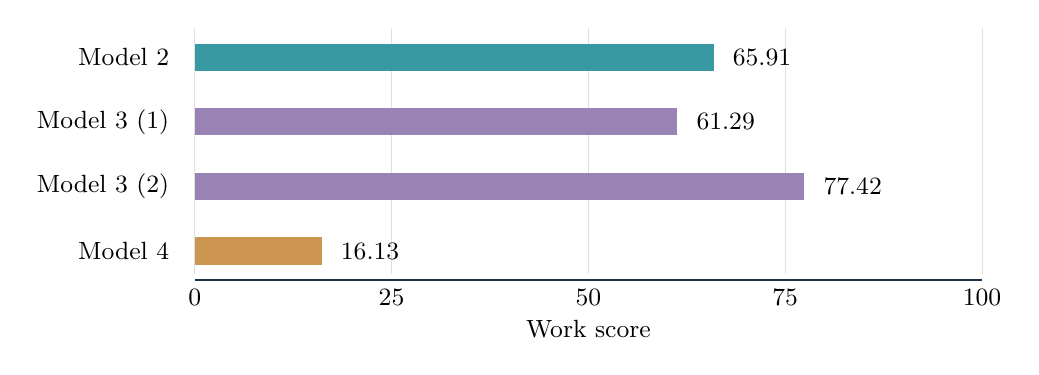
\begin{tikzpicture}[x=1cm,y=.82cm]
\foreach \x in {0,2.5,5,7.5,10} \draw[black!12] (\x,-.35)--(\x,3.45);
\foreach \y/\name/\value/\col/\display in {3/Model 2/65.91/Teal/65.91,2/Model 3 (1)/61.29/Purple/61.29,1/Model 3 (2)/77.42/Purple/77.42,0/Model 4/16.13/Amber/16.13} {
 \node[anchor=east,font=\small] at (-.2,\y) {\name};
 \fill[\col!80] (0,{\y-.21}) rectangle ({\value/10},{\y+.21});
 \node[anchor=west,font=\small] at ({\value/10+.12},\y) {\display};
}
\draw[Ink] (0,-.45)--(10,-.45);
\foreach \x/\label in {0/0,2.5/25,5/50,7.5/75,10/100} \node[below,font=\small] at (\x,-.45) {\label};
\node[below,font=\small] at (5,-.92) {Work score};
\end{tikzpicture}
\end{center}
\reportcaption{Figure 7. Verified work across four Case 2 attempts.}

No attempt passed the complete investigation. Only Model 2 submitted a final recommendation. Models 3 and 4 did not finish. Model 3's two bars represent separate attempts, not two agents or a measured improvement caused by training.

\begin{tabularx}{\textwidth}{@{}Ylrr@{}}\toprule
Agent / attempt & Final outcome & API requests & Cost (USD) \\\midrule
Model 2 & Submitted, but failed checks & 53 & 1.17 \\
Model 3, attempt 1 & Did not submit & 65 & 7.39 \\
Model 3, attempt 2 & Did not submit & 65 & 8.80 \\
Model 4 & Did not submit & 65 & 0.88 \\\bottomrule
\end{tabularx}
\reportcaption{Table 3. Completion and inference cost.}

Case 2 assigns partial scores to verifiable unfinished work. Case 1 did not score its unfinished attempt. This difference prevents a direct comparison of case-average scores. Model 1 did not take part in this Case 2 comparison.

\reporthead{The combined result concealed a site problem}
The next chart compares ranking across all patients with ranking at the weakest site. AUC 0.50 means chance ranking. The agents used different accepted patient selections, so their exact estimates differ.

\begin{center}
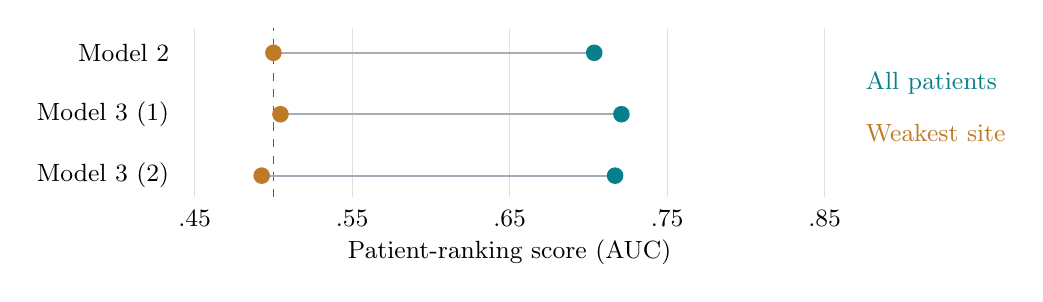
\begin{tikzpicture}[x=1cm,y=.78cm]
\foreach \x/\label in {0/.45,2/.55,4/.65,6/.75,8/.85} {
 \draw[black!12] (\x,-.35)--(\x,2.4);
 \node[below,font=\small] at (\x,-.4) {\label};
}
\draw[Muted,dashed] (1,-.35)--(1,2.4);
\foreach \y/\name/\all/\weak in {2/Model 2/.703704/.500000,1/Model 3 (1)/.720982/.504464,0/Model 3 (2)/.716964/.492560} {
 \node[anchor=east,font=\small] at (-.2,\y) {\name};
 \draw[Ink!40,thick] ({(\weak-.45)*20},\y)--({(\all-.45)*20},\y);
 \fill[Amber] ({(\weak-.45)*20},\y) circle (3pt);
 \fill[Teal] ({(\all-.45)*20},\y) circle (3pt);
}
\node[below,font=\small] at (4,-.88) {Patient-ranking score (AUC)};
\node[font=\small,anchor=west] at (8.4,1.5) {\textcolor{Teal}{All patients}};
\node[font=\small,anchor=west] at (8.4,.7) {\textcolor{Amber}{Weakest site}};
\end{tikzpicture}
\end{center}
\reportcaption{Figure 8. Overall ranking versus the weakest study site.}

Across all patients, AUC was about 0.70--0.72. At the weakest site, it was about 0.50. This gap limits claims about reliable performance across sites. It does not, by itself, identify the cause.

The additional cohort also provided mixed information. Its AUC was 0.672, but its net benefit at the 50\% cutoff was $-0.087$. Better knowledge of ranking did not establish that the proposed cutoff was useful.

\newpage
\reportcase{2}{The failures occurred at different steps}
The map separates checks that failed from work that was missing. A missing entry does not prove an incorrect calculation. It means that the evaluator could not find qualifying work for that check.

\begin{tabularx}{\textwidth}{@{}Ycccc@{}}\toprule
What the evaluator checked & M2 & M3 (1) & M3 (2) & M4 \\\midrule
Kept the plan fixed after seeing responses & \reportfailed & \reportmet & \reportmet & \reportmet \\
Provided the required links between saved files & \reportfailed & \reportmet & \reportmet & \reportmissing \\
Handled repeated records from the same patient & \reportmet & \reportmet & \reportmet & \reportmissing \\
Supported patient ranking and its uncertainty & \reportmet & \reportfailed & \reportmet & \reportmissing \\
Checked whether predicted chances matched responses & \reportmet & \reportmet & \reportmet & \reportmissing \\
Checked the consequences of the 50\% cutoff & \reportmet & \reportmet & \reportmet & \reportmissing \\
Checked patient and record counts at each site & \reportfailed & \reportfailed & \reportfailed & \reportmissing \\
Used the purchased information to support a decision & \reportfailed & \reportfailed & \reportfailed & \reportmissing \\
Supported the final recommendation & \reportfailed & \reportmissing & \reportmissing & \reportmissing \\\bottomrule
\end{tabularx}
\reportcaption{Figure 9. Where each Case 2 investigation failed or stopped.}

Green means the check passed. Amber means it failed. Grey means qualifying work was missing. M2--M4 abbreviate Model 2--Model 4. Parentheses identify Model 3's two attempts.

\reporthead{Model 2 changed a declared input after seeing responses}
Model 2 calculated several primary numbers correctly. It bought another cohort, reduced its stated confidence in site performance and submitted a stop decision. However, it changed a declared input file after the response results were available. That was the first important error.

The saved work no longer demonstrated that the final analysis followed the original plan. Additional broken file links and decision-rule inconsistencies also remained. The cautious final recommendation did not fix those problems. An input-protection tool could help, but no paired test measured its effect.

\reporthead{Model 3's first attempt omitted required uncertainty}
The agent calculated useful point estimates but omitted the required uncertainty estimate for ranking. It also left the site analysis and purchased-cohort analysis incomplete. It did not submit. This is a specific omission, not evidence that all its calculations were wrong.

\reporthead{Model 3's second attempt confused records with people}
This attempt supplied the required ranking uncertainty. Its first important error was the site count. It reported 24 records where there were 30 records from 24 patient groups. At the other sites, it reported 14 instead of 36 records and 58 instead of 137.

The mistake hid repeated sampling. Correct AUC values did not make the count audit correct. The agent later omitted the additional cohort's negative net benefit and drafted a decision outside its previously stated rules. It wrote a submission script but never executed it.

\reporthead{Model 4 did not deliver enough finished work for a scientific diagnosis}
Model 4 reached response disclosure and continued working. It did not register qualifying calculations or finish the purchase and recommendation stages. No specific important scientific error was established before it stopped. The observed problem was incomplete delivery of the investigation.

\reporthead{Interpretation}
Case 2 exposes errors in plan adherence, uncertainty, patient counting and use of additional data. However, three unfinished attempts also indicate a completion problem. The results do not establish a purely scientific difficulty level or a stable model ranking. Statistical assistance and workflow tools should be tested separately before attributing the failures to model training.

\newpage
\reportcase{3}{Can the team check how the predictions were produced?}
Cases 1 and 2 ask whether the analysis supports a recommendation. Case 3 examines an earlier link: whether the prediction file came from a procedure that the team can check. A reported result can be reproduced numerically without establishing how its predictions were generated.

This case contains 122 records from 112 provisional patient groups. Ten groups contain repeated records, and two response records disagree with the central review. The agent receives original predictions, processing code, fitting records and logs. It must distinguish what these files establish from what remains unknown.

\reporthead{Two questions, not one}
First, the agent calculates how well the original predictions match patient responses. Second, it checks whether the documented processing supports treating those predictions as valid study results. A high AUC answers the first question but not the second.

The agent can request a new, traceable execution. That package contains the model, inputs, fitted preprocessing information and resulting predictions. Two conditions begin with identical files but provide different execution results. The agent cannot know which result it will receive from the initial packet.

\begin{center}
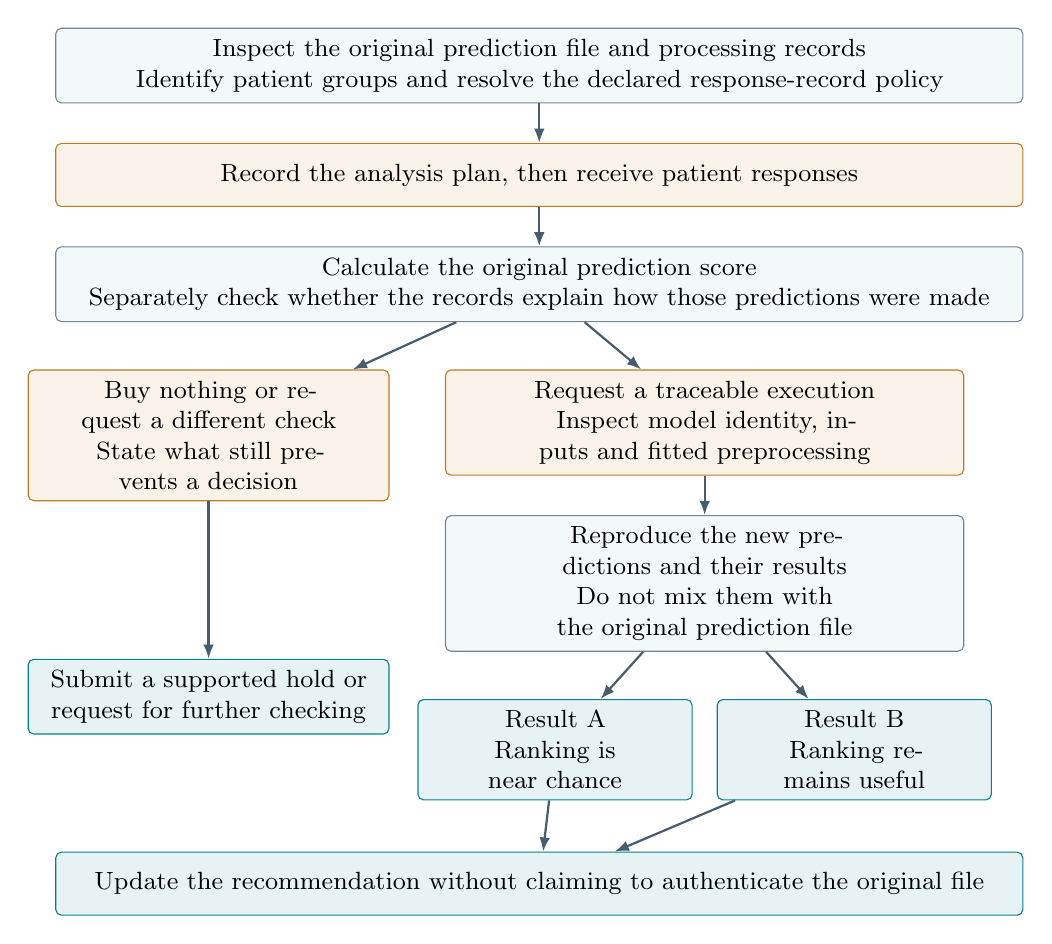
\begin{tikzpicture}[node distance=5mm]
\node[box] (a) {Inspect the original prediction file and processing records\\Identify patient groups and resolve the declared response-record policy};
\node[gate,below=of a] (b) {Record the analysis plan, then receive patient responses};
\node[box,below=of b] (c) {Calculate the original prediction score\\Separately check whether the records explain how those predictions were made};
\node[gate,text width=4.3cm,below=6mm of c.south,xshift=-4.2cm] (d) {Buy nothing or request a different check\\State what still prevents a decision};
\node[gate,text width=6.3cm,below=6mm of c.south,xshift=2.1cm] (e) {Request a traceable execution\\Inspect model identity, inputs and fitted preprocessing};
\node[box,text width=6.3cm,below=of e] (f) {Reproduce the new predictions and their results\\Do not mix them with the original prediction file};
\node[result,text width=3.2cm,below=6mm of f.south,xshift=-1.9cm] (g) {Result A\\Ranking is near chance};
\node[result,text width=3.2cm,below=6mm of f.south,xshift=1.9cm] (h) {Result B\\Ranking remains useful};
\node[result,text width=4.3cm,below=20mm of d] (i) {Submit a supported hold or request for further checking};
\node[result,anchor=north] (j) at ($(g.south)!0.5!(h.south)+(-2.1,-.65)$) {Update the recommendation without claiming to authenticate the original file};
\foreach \x/\y in {a/b,b/c,c/d,c/e,d/i,e/f,f/g,f/h,g/j,h/j} \draw[arr] (\x)--(\y);
\end{tikzpicture}
\end{center}
\reportcaption{Figure 10. Checking prediction history and a new execution.}

A supported decision to hold the study can pass without buying the execution. If the agent buys it, the agent must reproduce and interpret the returned calculations. A successful new execution does not establish the origin of the old file.

\newpage
\reportcase{3}{The available results imply different next steps}
\reportstatus{Reference calculations only. Comparable AI-agent results are not yet available.}
The reference execution uses a fixed logistic predictor and three input features. These represent an interferon score, an epithelial score and log library size. The preprocessing uses means and standard deviations from 180 training rows. The files let an analyst reproduce the predicted probabilities.

\begin{center}
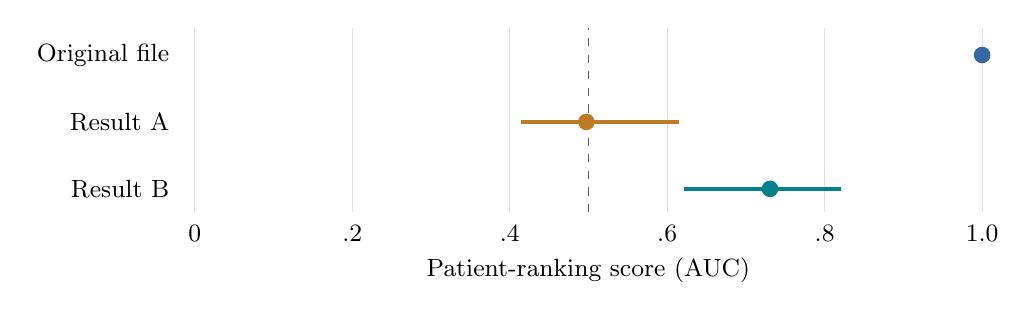
\begin{tikzpicture}[x=1cm,y=.85cm]
\foreach \x/\label in {0/0,2/.2,4/.4,6/.6,8/.8,10/1.0} {
 \draw[black!12] (\x,-.35)--(\x,2.4);
 \node[below,font=\small] at (\x,-.4) {\label};
}
\draw[Muted,dashed] (5,-.35)--(5,2.4);
\foreach \y/\name/\mid/\low/\high/\col in {2/Original file/1/1/1/Blue,1/Result A/.49736/.41394/.61474/Amber,0/Result B/.73057/.62194/.82071/Teal} {
 \node[anchor=east,font=\small] at (-.2,\y) {\name};
 \draw[\col,line width=1.3pt] ({\low*10},\y)--({\high*10},\y);
 \fill[\col] ({\mid*10},\y) circle (3pt);
}
\node[below,font=\small] at (5,-.88) {Patient-ranking score (AUC)};
\end{tikzpicture}
\end{center}
\reportcaption{Figure 11. Reference ranking estimates and 95\% intervals.}

The original prediction file has AUC 1.00. That perfect result does not prove a valid prediction history. Result A has AUC about 0.50, which provides no useful ranking in this sample. Result B has AUC 0.731, which supports a more favourable assessment of ranking.

To estimate uncertainty, the reference analysis repeatedly samples patients from the available data. Records from the same patient stay together. The analysis used 100 such samples. These are controlled reference calculations, not a clinical performance estimate.

\begin{tabularx}{\textwidth}{@{}Yrrr@{}}\toprule
Quantity & Original file & Result A & Result B \\\midrule
Patient ranking: AUC & 1.000 & 0.497 & 0.731 \\
Probability error: Brier score & 0.015 & 0.299 & 0.207 \\
Mismatch between chances and responses: calibration error & 0.111 & 0.231 & 0.122 \\
Performance of the 50\% cutoff: net benefit & 0.411 & $-0.027$ & 0.080 \\\bottomrule
\end{tabularx}
\reportcaption{Table 4. Reference calculations for the two execution results.}

Result B does not support every proposed use. Its calibration error is 0.12186, just above the case's stated limit of 0.12. It can therefore support a restricted next research study without automatically supporting use of the predicted probabilities.

\reporthead{What the agent must not conclude}
The two execution results differ in the association between patient features and responses. They do not differ only in one processing step. The comparison therefore cannot prove that removing information leakage caused the decline in ranking.

Similarly, a result near chance does not prove that predicting anti-TNF response is biologically impossible. A useful new result does not repair missing documentation for the original predictions. These are the limits the agent must preserve when it recommends the next step.

\reporthead{What is known so far}
Six reference solutions satisfy the local checks across the two results and three supported analysis methods. There are no comparable AI-agent attempts for this specification. Scores, completion rates, inference costs and model-specific failures remain unmeasured.

Case 4 extends this distinction between claims. Even when ranking is useful and the prediction procedure is clear, the proposed probability cutoff may still perform poorly.

\newpage
\reportcase{4}{Do useful rankings support the proposed cutoff?}
The sponsor reports an AUC near 0.74 and proposes flagging patients whose predicted response chance exceeds 50\%. The agent must test that proposal. A predictor can put likely responders above likely nonresponders while assigning inaccurate chances to both groups.

This case contains 158 records from 148 people across three study sites. Two noncritical covariates are missing. The agent receives predictions, patient and response records, processing documents and access to a matched external cohort.

\reporthead{Why the distinction matters}
Ranking asks whether responders tend to receive higher scores. Calibration asks whether the numerical chances are right. The cutoff question asks what happens when those chances trigger a decision. These are separate tests, so one favourable score cannot substitute for the others.

For example, predicted chances might all be too high while retaining the correct patient order. AUC could remain high, yet the 50\% cutoff could flag too many nonresponders. This example explains the distinction, not a measured mechanism in this case.

\begin{center}
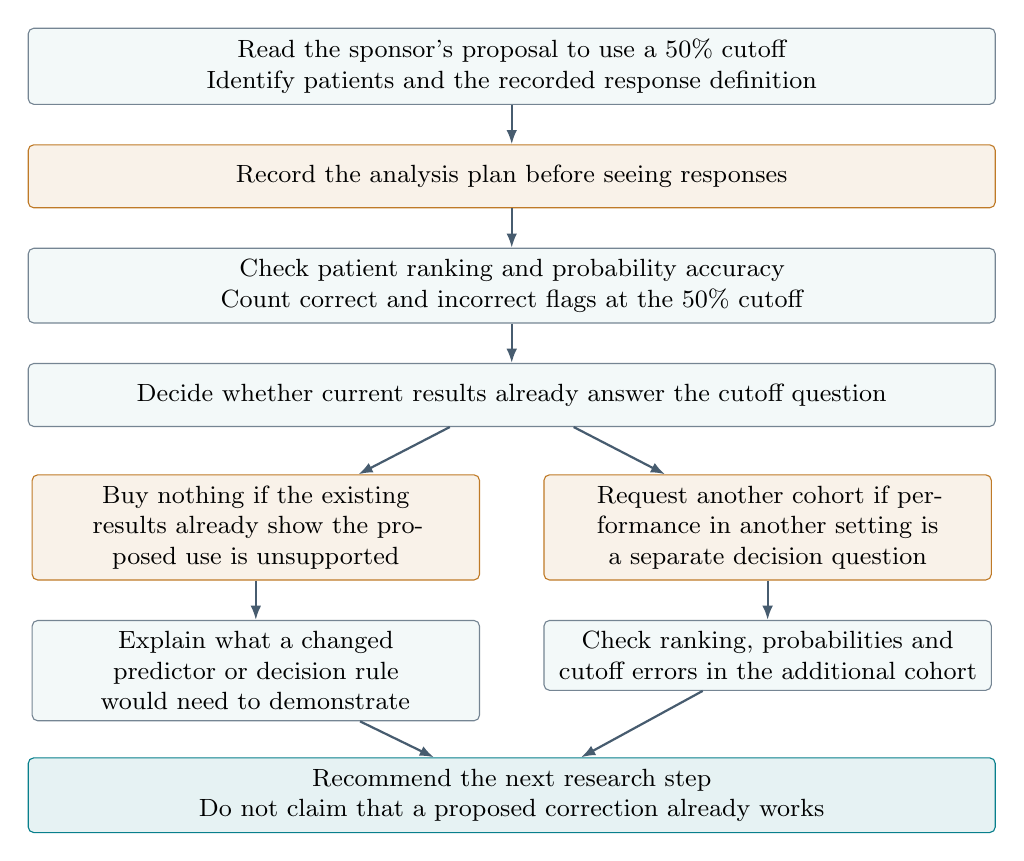
\begin{tikzpicture}[node distance=5mm]
\node[box] (a) {Read the sponsor's proposal to use a 50\% cutoff\\Identify patients and the recorded response definition};
\node[gate,below=of a] (b) {Record the analysis plan before seeing responses};
\node[box,below=of b] (c) {Check patient ranking and probability accuracy\\Count correct and incorrect flags at the 50\% cutoff};
\node[box,below=of c] (d) {Decide whether current results already answer the cutoff question};
\node[gate,text width=5.4cm,below=6mm of d.south,xshift=-3.25cm] (e) {Buy nothing if the existing results already show the proposed use is unsupported};
\node[gate,text width=5.4cm,below=6mm of d.south,xshift=3.25cm] (f) {Request another cohort if performance in another setting is a separate decision question};
\node[box,text width=5.4cm,below=of e] (g) {Explain what a changed predictor or decision rule would need to demonstrate};
\node[box,text width=5.4cm,below=of f] (h) {Check ranking, probabilities and cutoff errors in the additional cohort};
\node[result,anchor=north] (i) at ($(g.south)!0.5!(h.south)+(0,-.65)$) {Recommend the next research step\\Do not claim that a proposed correction already works};
\foreach \x/\y in {a/b,b/c,c/d,d/e,d/f,e/g,f/h,g/i,h/i} \draw[arr] (\x)--(\y);
\end{tikzpicture}
\end{center}
\reportcaption{Figure 12. Testing the proposed cutoff before requesting more data.}

The agent can reject the current cutoff without abandoning the entire research programme. Adjusting the probabilities and testing them independently could be a next investment. The case does not demonstrate that this adjustment works.

A second cohort is not always necessary for the immediate decision. If current results already reject the proposed use, another purchase needs a separate purpose. The scoring rules for this further study still need to confirm both decision paths.

\newpage
\reportcase{4}{Better ranking did not resolve the cutoff problem}
\reportstatus{Provisional reference values only. No comparable AI-agent results.}
The available numbers show why an AUC-only review would be incomplete. The second cohort has better ranking, but the proposed cutoff still performs poorly. The two charts use different scales because they measure different things.

\begin{center}
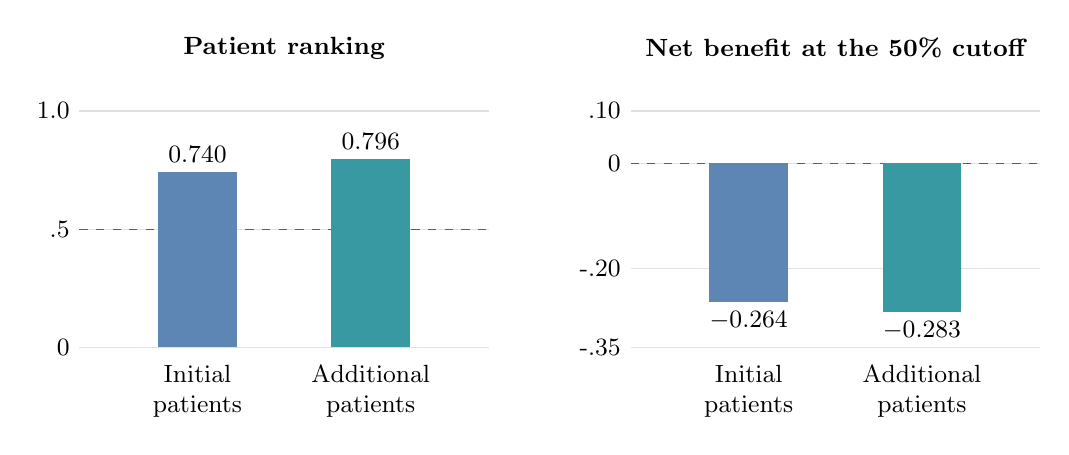
\begin{tikzpicture}[x=1cm,y=1cm]
\node[font=\small\bfseries] at (2.6,3.8) {Patient ranking};
\node[font=\small\bfseries] at (9.6,3.8) {Net benefit at the 50\% cutoff};
% Ranking panel: 0 to 1.
\foreach \y/\label in {0/0,1.5/.5,3/1.0} {
 \draw[black!12] (0,\y)--(5.2,\y);
 \node[left,font=\small] at (0,\y) {\label};
}
\draw[Muted,dashed] (0,1.5)--(5.2,1.5);
\fill[Blue!80] (1,0) rectangle (2,{.739713*3});
\fill[Teal!80] (3.2,0) rectangle (4.2,{.796037*3});
\node[above,font=\small] at (1.5,{.739713*3}) {0.740};
\node[above,font=\small] at (3.7,{.796037*3}) {0.796};
\node[below,align=center,font=\small] at (1.5,-.1) {Initial\\patients};
\node[below,align=center,font=\small] at (3.7,-.1) {Additional\\patients};
% Net benefit panel: -.35 to .1.
\foreach \y/\label in {0/-.35,1/-.20,2.333/0,3/.10} {
 \draw[black!12] (7,\y)--(12.2,\y);
 \node[left,font=\small] at (7,\y) {\label};
}
\draw[Muted,dashed] (7,2.333)--(12.2,2.333);
\fill[Blue!80] (8,{(-.263514+.35)/.45*3}) rectangle (9,2.333);
\fill[Teal!80] (10.2,{(-.282609+.35)/.45*3}) rectangle (11.2,2.333);
\node[below,font=\small] at (8.5,{(-.263514+.35)/.45*3}) {$-0.264$};
\node[below,font=\small] at (10.7,{(-.282609+.35)/.45*3}) {$-0.283$};
\node[below,align=center,font=\small] at (8.5,-.1) {Initial\\patients};
\node[below,align=center,font=\small] at (10.7,-.1) {Additional\\patients};
\end{tikzpicture}
\end{center}
\reportcaption{Figure 13. Higher AUC with persistently negative net benefit.}

At the 50\% cutoff, this calculation gives equal weight to a correct positive prediction and an incorrect positive prediction. A negative result means the incorrect flags outweigh the correct flags under that rule. The comparison is against flagging nobody. It is not a demonstrated effect on patient health.

\begin{tabularx}{\textwidth}{@{}Yrr@{}}\toprule
Quantity & Initial patients & Additional patients \\\midrule
Patient ranking: AUC & 0.740 & 0.796 \\
Reported AUC interval & [0.651, 0.824] & [0.683, 0.891] \\
Probability error: Brier score & 0.332 & 0.327 \\
Mismatch between chances and responses: calibration error & 0.404 & 0.405 \\
Performance of the 50\% cutoff: net benefit & $-0.264$ & $-0.283$ \\\bottomrule
\end{tabularx}
\reportcaption{Table 5. Available Case 4 reference values.}

The case's stated research rules require AUC at least 0.70 and an uncertainty lower limit at least 0.58. They also limit Brier score to 0.23 and calibration error to 0.12, and require nonnegative net benefit. These are exercise-specific criteria, not universal clinical standards.

The available values satisfy the ranking rules but fail the probability and cutoff rules. More data clarified the picture without resolving the problem. Before agent evaluation, an independent calculation must confirm these provisional values and both allowed purchase paths.

\reporthead{What the four cases measure together}
The shared task is to connect patient records, calculations and a defensible research recommendation. Case 1 demonstrates complete solutions and identifiable failures. Case 2 exposes additional errors, but unfinished attempts also limit the conclusions. Cases 3 and 4 define further tests without supplying measured agent results.

The current observations do not establish a stable ranking of AI models. They also do not identify a need for more training data, expert demonstrations or reinforcement learning. Those explanations require repeated attempts and direct tests of the proposed assistance.

\vfill
\begingroup\footnotesize\color{Muted}
\textbf{Model key.} Model 1: GPT-5. Model 2: GPT-5.1. Model 3: Claude Sonnet 4. Model 4: Gemini 3.1 Pro Preview. Identifiers stay fixed across cases and do not indicate rank.
\par\textbf{Scope.} Results use the accepted reports and saved outputs through 14 September 2026. Case 2 uses its final scoring rules. No new model attempt occurred during report preparation. These controlled exercises do not establish clinical validity.
\par\endgroup
\end{document}
